\documentclass[expanded]{lkx_pset}

\title{Math 213b Problem Set 9}
\author{Lev Kruglyak}
\due{April 10, 2024}

\usepackage{graphicx}

\newcommand{\D}{\mathbb{D}}
\newcommand{\x}{\mathbf{x}}
\usepackage{pgfplots}
\pgfplotsset{
	compat=1.12,
}

\newcommand{\dd}{\partial}
\newcommand{\ddc}{\overline{\partial}}

\usepackage{bbm}
\newcommand{\bbDelta}{\bm{\Delta}}


\collaborator{AJ LaMotta}
\collaborator{Jarell Cheong}

\begin{document}
\maketitle

\begin{problem}{1}
Recall the doubly-periodic surface $X$ which appeared on the first problem set. Previously, you thought about the topology of submanifolds of $X$. Consider now that $X$ is a Riemann surface, so that the double periodicity is by holomorphic maps from $X$ to itself. Let $\{p_{1}, \dots p_{n}\}$ be any finite subset of $X$. Show that there is a bounded holomorphic differential on $X$ that vanishes at all the points $p_{i}$ and is not identically zero.
\end{problem}

\begin{solution}
	Let $G$ be the group $G = m\Z\oplus m\Z$. This group acts by translation on $X$, and we get a holomorphic quotient map $X \to X/G$. This quotient surface has $(m-1)^2$ holes in its fundamental domain, and the quotient relation glues on an additional $2m$ handles. This means that $X/G$ has genus $M=2m+(m-1)^2$. Let's fix some $m$ which sets $M>n$.

	Now let $q_1,\ldots,q_n$ be translations of the original points $p_1,\ldots, p_n$ to be in some fixed fundamental domain. We then get a $\C$-linear map
	\[
		\definefunction{\Phi}{H^{1,0}(X/G)\cong\C^M}{\C^n}{\alpha}{\alpha_{q_1}(1),\ldots, \alpha_{q_n}(1)}
	\]
	where $\alpha_{q_n} : T_{q_i}(X/G) \to \C$. By the rank-nullity theorem, it follows that $\dim\ker(\Phi)\geq M-n$ so there are $M-n$ holomorphic differentials $\alpha_1,\ldots, \alpha_{M_n}$ which are not identically zero and linearly independent, and vanishing on $q_1,\ldots, q_n$. Pulling these back along the covering map $\pi : X \to X/G$, we obtain (at least one) holomorphic differential $\omega = \pi^*\alpha_i$ on $X$ which vanishes at the preimages of $q_1,\ldots, q_n$. (Namely $p_1,\ldots p_n$) Since $X/G$ is a compact Riemann surface, it follows that $\alpha_i\in H^{1,0}(X/G)$ is bounded and so the pullback $\omega = \pi^*\alpha_i$ is bounded and satisfies the conditions of the problem.
\end{solution}

\begin{problem}{2}
Let $g(x)$ be a complex polynomial of degree $2g+2$ with distinct roots, say
\[
	g(x) = (x - \lambda_{1})(x - \lambda_{2}) \cdots (x-\lambda_{2g+2}).
\]
Let $X'$ be the branched double cover of $\C$ described by the equation $y^{2}=g(x)$ in $\C^{2}$, and let $X \to \CP^{1}$ be obtained by completing the branched covering in the standard way (i.e.\ just as any proper map of Riemann surfaces $X'\to Y'=Y-\{q_{1},\dots, q_{r}\}$ can be completed to a map $X\to Y$).\medskip
\end{problem}

\begin{parts}
	\begin{part}{}
		What is the genus of $X$?
	\end{part}

	Let $\pi : X' \to \C$ be the branched double cover described in the problem. The branch points of this cover are by construction the points $(\lambda_1, 0),\ldots, (\lambda_{2g+2},0)$ with corresponding ramification points $\lambda_1,\ldots,\lambda_{2g+2}$. After completion to $\CP^1$, which we'll call $\widetilde{\pi} : X' \to \CP^1$, we can have up to one more ramification $\infty\in\CP^1$, so the number of ramification points is either $2g+2$ or $2g+3$. However, since $\deg(\widetilde{\pi})=2$, the Riemann-Hurwitz theorem gives us
	\[
		R_{\widetilde{\pi}} = 2g_X - 2 - 2(2g_{\CP^1} - 2) = 2g_X +2
	\]
	where $R_{\widetilde{\pi}}$ is the number of ramification points of $\widetilde{\pi}$. This means that $R_{\widetilde{\pi}}$ is even and so equals $2g+2$. This then implies that $g_X=g$ so the genus of $X$ is $g$.

	\begin{part}{}
		Show that the meromorphic form $(dx)/y$ on $X'$ actually extends to a holomorphic form $\alpha_{1}$ on all of $X$. (You can refer to your result on Problem Set 6.) Where are the zeros of $\alpha_{1}$ and what are their multiplicities?\medskip
	\end{part}

	Consider the polynomial
	\[
		F(x,y) = y^2 - g(x) \quad\implies\quad \frac{\partial F}{\partial x} = -g'(x),\quad \frac{\partial F}{\partial y} = 2y.
	\]
	Since $F$ has a nonvanishing gradient at each point, it follows from the results of previous problem sets that $X'$ is in fact a Riemann surface. Using Problem 4 on Homework 6, we can set $G(x,y)=\partial F/\partial y = 2y$ and $\alpha = G(x,y)^{-1}\,dx = dx/2y$. Then $\alpha$ is a well-defined nowhere zero holomorphic differential on $X'$, so $\alpha_1=2\alpha = dx/y$ is also a well-defined nowhere zero holomorphic differential on $X'$.

	To understand the zeroes of $\alpha_1$, recall that
	\[
		2g-2 = \sum_{p\in X}\textrm{ord}_p(\alpha_1)=\textrm{ord}_{\infty_1}(\alpha_1) + \textrm{ord}_{\infty_2}(\alpha)_1
	\]
	By symmetry, it then follows that $\textrm{ord}_{\infty_1}(\alpha_1) = \textrm{ord}_{\infty_2}(\alpha_1) = g-1$, so the zeros of $\alpha_1$ are exactly $\infty_1,\infty_2$, each of multiplicity $g-1$.

	\begin{part}{}
		Show that the forms $\alpha_{i} = x^{i-1}\alpha_{1}$ for $i=1,\dots, g$ are a basis for $H^{1,0}(X)$.
	\end{part}
	Clearly, we have
	\[
		\textrm{ord}_{\infty_j}(x^{i-1}\alpha_1) = \ord_{\infty_j}(x^{i-1}) + \textrm{ord}_{\infty_j}(\alpha_1) = -(i-1)+g-1) = g-i\geq 0
	\]
	so $x^{i-1}\alpha_1$ is holomorphic on all of $X$ and thus $\alpha_1,\ldots, \alpha_g\in H^{1,0}(X)$. They are clearly linearly independent, and since $\dim H^{1,0}(X)=g$, we can conclude that $\alpha_1,\ldots, \alpha_g$ form a basis for $H^{1,0}(X)$.
\end{parts}

\begin{problem}{3}
Let $X$ be the same hyperelliptic curve as in the previous question, but for clarity now take the roots  $\lambda_{i}$ to be real and increasing:
\[
	\lambda_{1} < \lambda_{2} < \dots < \lambda_{2g+2}.
\]
In the next question it will be convenient to take them to be equally spaced and symmetric about zero: specifically, $\lambda_{i}= -2g-3+2i$, which is the sequence,
\[
	-2g-1, -2g+1, \dots -1, 1, \dots , 2g-1, 2g+1.
\]
Any sequence of increasing real numbers would do
here but we want something specific for the calculations later.
\end{problem}

\begin{parts}
	\begin{part}{}
		On the real axis, where is $g(x)$ positive?
	\end{part}

	On the real axis, the function $g(x)$ is positive if and only if $x$ is less than evenly many of the $\lambda_i$'s, or equivalently,
	\[
		x\in (-\infty, -2g-1)\cup (2g+1,\infty)\cup \bigcup^g_{j=1}(-2g+4j-3, -2g+4j-1).
	\]

	\begin{part}{}
		Exhibit on $X$ a standard set of $a$ and $b$ curves $a_{1},\dots , a_{g}$ and $b_{1},\dots, b_{g}$ by drawing their images in $\C$ (the $x$ coordinate) and explaining how to lift these images to $X$. It may help to remember that the collection of $a$ and $b$ curves is far from unique and that your curves win provided only that the curves have the correct intersection pattern.
	\end{part}

	Consider the following images in $\C$ of our $a$ and $b$ curves:
	\begin{center}
		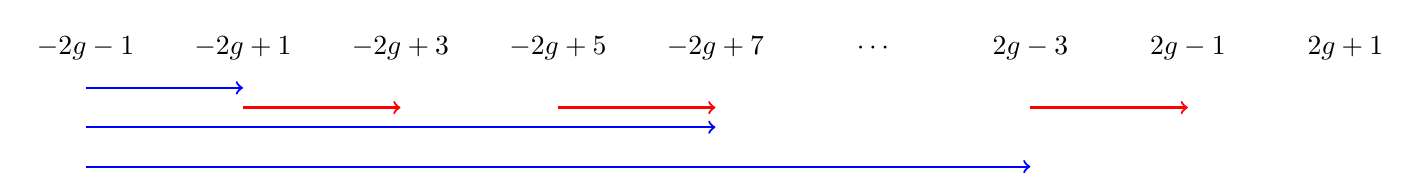
\begin{tikzpicture}
			\node (a) at (0,0) {$-2g-1$};
			\node (b) at (2,0) {$-2g+1$};
			\node (c) at (4,0) {$-2g+3$};
			\node (d) at (6,0) {$-2g+5$};
			\node (f) at (8,0) {$-2g+7$};
			\node (g) at (10,0) {$\cdots$};
			\node (h) at (12,0) {$2g-3$};
			\node (i) at (14,0) {$2g-1$};
			\node (j) at (16,0) {$2g+1$};

			\draw[blue, thick, ->] (0,-0.5) -- (2, -0.5);
			\draw[red, thick, ->] (2,-0.75) -- (4, -0.75);
			\draw[blue, thick, ->] (0,-1.0) -- (8, -1.0);
			\draw[red, thick, ->] (6,-0.75) -- (8, -0.75);
			\draw[blue, thick, ->] (0,-1.5) -- (12, -1.5);
			\draw[red, thick, ->] (12,-0.75) -- (14, -0.75);
		\end{tikzpicture}
	\end{center}

	In words, $a_j$ loops clockwise around $-2g+4j-3$ and $-2g+4j-1$, while $b_j$ loops anticlockwise around $-2g-1$ and $-2g+4j-3$. We can then lift the images of these curves by specifying basepoints and taking the unique lift that passes through these basepoints to $X$. Note that each $a_j$ intersects exactly one $b_j$, and they intersect at most twice. This means that they will have the correct intersection pattern in the lift.
\end{parts}

\begin{problem}{4}
Continuing the previous two problems, consider now the $A$- and $B$-periods of the forms $\alpha_{i}$.
\end{problem}

\begin{parts}
	\begin{part}{}Adjusting your $a$ and $b$ curves if necessary and relabelling, show that you can arrange that all the $A$-periods of all the $\alpha_{i}$ are real numbers, and write down explicit real definite integrals which compute them.\medskip
	\end{part}

	Since all of the $\alpha_i$'s are closed, given some $i,j$ and the results from the previous parts, we get
	\[
		\begin{aligned}
			A_j(\alpha_i) & = \int_{a_j}\frac{x^{i-1}\, dx}{y}                                                                                                                                               \\
			              & = \int_{-2g+4j-3}^{-2g+4j-1}\frac{x^{i-1}\, dx}{\sqrt{\prod_{k=1}^{2g+2}(x-(-2g-3+2k))}}+\int_{-2g+4j-1}^{-2g+4j-3}\frac{x^{i-1}\, dx}{-\sqrt{\prod_{k=1}^{2g+2}(x-(-2g-3+2k))}} \\
			              & = 2\int_{-2g+4j-3}^{-2g+4j-1}\frac{x^{i-1}\, dx}{\sqrt{\prod_{k=1}^{2g+2}(x-(-2g-3+2k))}}.
		\end{aligned}
	\]
	Each of these integrals is real since we are integrating over regions where $g(x)>0$ and so the square root in the denominator is well-defined.

	\begin{part}{}
		In the case $g=2$, with $\lambda_{i}$ as illustrated above,
		compute the integrals $A_{j}(\alpha_{i})$ by direct numerical integration (using any computing tool you like).
	\end{part}
	In the case when $g=2$, using Mathematica we obtain:
	\[
		\begin{aligned}
			A_{11} & = A_1(\alpha_1)=2\int_{-3}^{-1}\frac{dx}{\sqrt{(x^2-25)(x^2-9)(x^2-1)}}\approx 0.370162,        \\
			A_{12} & = A_2(\alpha_1) =2\int_1^3 \frac{dx}{\sqrt{(x^2-25)(x^2-9)(x^2-1)}}\approx 0.370162,            \\
			A_{21} & = A_1(\alpha_2) = 2\int_{-3}^{-1}\frac{x\, dx}{\sqrt{(x^2-25)(x^2-9)(x^2-1)}}\approx -0.707869, \\
			A_{22} & = A_2(\alpha_2) =2\int_1^3 \frac{x\, dx}{\sqrt{(x^2-25)(x^2-9)(x^2-1)}}\approx 0.707869.
		\end{aligned}
	\]

	\begin{part}{}
		Put them in a 2-by-2 matrix, then compute a normalized basis for the holomorphic differentials with respect to your $a$-curves. That is, find $\widetilde\alpha_{1}$ and $\widetilde\alpha_{2}$ with $A_{j}(\widetilde\alpha_{i})=\delta_{ij}$.\medskip
	\end{part}

	Putting the results of the previous section into matrix form, we get
	\[
		\begin{pmatrix}
			0.370162  & 0.370162 \\
			-0.707869 & 0.707869
		\end{pmatrix}.
	\]
	The normalized basis then becomes
	\[
		\begin{aligned}
			\widetilde{\alpha_1} & = 1.35076\alpha_1-0.706345\alpha_2, \\
			\widetilde{\alpha_2} & = 1.35076\alpha_1+0.706345\alpha_2.
		\end{aligned}
	\]
	Using linearity of the period integrals $A_1$ and $A_2$ then yields $A_{ij}=A_j(\alpha_i)\approx \delta_{ij}$, so $\widetilde{\alpha_1},\widetilde{\alpha_2}$ is a normalized basis.

	\begin{part}{}
		Using your chosen $b$ curves, compute the $B$-periods of the normalized differentials numerically and verify the Riemann bilinear relations.
	\end{part}

	To compute the $B$-periods, let's modify the $a$ and $b$ curves to those whose images in $\C$ follow the following configuration:
	\begin{itemize}
		\item $b_1$ goes counterclockwise around $-5$ and $-3$,
		\item $b_2$ goes clockwise around $3$ and $5$,
		\item $a_1$ goes clockwise around $-3$ and $-1$,
		\item $a_2$ goes clockwise around $1$ and $3$,
	\end{itemize}
	With these new $a$ and $b$ curves, and keeping track of which branch of the square root we're integrating over with respect to the orientation of the $b$ curves, we see that the $B$-periods are:
	\[
		\begin{aligned}
			B_1(\alpha_1) & = 2\int_{-3}^{-5} \frac{dx}{\sqrt{(x^2-25)(x^2-9)(x^2-1)}}\approx 0.217891i,     \\
			B_2(\alpha_1) & = 2\int_5^3 \frac{dx}{\sqrt{(x^2-25)(x^2-9)(x^2-1)}}\approx 0.217891i,           \\
			B_1(\alpha_2) & = 2\int_{-3}^{-5}\frac{x\, dx}{\sqrt{(x^2-25)(x^2-9)(x^2-1)}}\approx -0.828319i, \\
			B_2(\alpha_2) & = 2\int_5^3 \frac{x\, dx}{\sqrt{(x^2-25)(x^2-9)(x^2-1)}}\approx 0.828319i.
		\end{aligned}
	\]
	With respect to the normalized basis we found earlier, we get
	\[
		B_{11}\approx 0.879397i,\quad B_{12}\approx -0.290761i,\quad B_{21}\approx -0.290761i,\quad B_{22}\approx 0.879397i,
	\]
	so the $B$-matrix is symmetric, and its imaginary part
	\[
		\begin{pmatrix}
			0.879397  & -0.290761 \\
			-0.290761 & 0.879397
		\end{pmatrix}
	\]
	has eigenvalues $\lambda_1\approx 1.17016$ and $\lambda_2\approx 0.588636$. We can conclude that the $B$-matrix is positive definite.
\end{parts}

\end{document}
